\documentclass{amsart}
\usepackage{tikz}
\usepackage{float}

\usepackage{amsmath}
\usepackage{amsfonts}
\usepackage{amsthm}
\usepackage{enumitem}
\usepackage{dsfont}
\usepackage{amssymb}
\usepackage{pifont}
\usepackage{mathtools}

\newtheorem{thm}{Theorem}[section]
\newtheorem{lem}[thm]{Lemma}
\newtheorem{prop}[thm]{Proposition}
\newtheorem{conj}[thm]{Conjecture}
\newtheorem{cor}[thm]{Corollary}

\newtheorem*{prop*}{Proposition}

\theoremstyle{definition}
\newtheorem{claim}[thm]{Claim}
\newtheorem{defn}[thm]{Definition}
\newtheorem{quest}[thm]{Question}
\newtheorem{remark}[thm]{Remark}
\newtheorem{fact}[thm]{Fact}
\newtheorem{note}[thm]{Note}

\newtheorem*{claim*}{Claim}
\newtheorem*{quest*}{Question}
\newtheorem*{remark*}{Remark}
\newtheorem*{fact*}{Fact}

\newcommand{\N}{\ensuremath{\mathbb{N}}}
\newcommand{\Z}{\ensuremath{\mathbb{Z}}}
\newcommand{\Q}{\ensuremath{\mathbb{Q}}}
\newcommand{\R}{\ensuremath{\mathbb{R}}}
\newcommand{\C}{\ensuremath{\mathbb{C}}}
\newcommand{\F}{\ensuremath{\mathbb{F}}}
\newcommand{\AP}{\ensuremath{\mathcal{A}_{2^{n}}}}
\newcommand{\BP}{\ensuremath{\mathcal{B}_{2^{n}}}}
\newcommand{\CP}{\ensuremath{\mathcal{C}_{2^{n}}}}
\newcommand{\DP}{\ensuremath{\mathcal{D}_{2^{n}}}}
\newcommand{\EP}{\ensuremath{\mathcal{E}_{2^{n}}}}
\newcommand{\FP}{\ensuremath{\mathcal{F}_{2^{n}}}}

\newcommand{\E}{\ensuremath{\mathbb{E}}}
\newcommand{\1}{\ensuremath{\mathds{1}}}

\newcommand{\pair}[2]{\ensuremath{\langle #1, #2 \rangle}}

\DeclareMathOperator{\Gal}{Gal}
\DeclareMathOperator{\Jac}{Jac}
\DeclareMathOperator{\Var}{Var}
\DeclareMathOperator{\Cov}{Cov}
\DeclareMathOperator{\Div}{Div}
\DeclareMathOperator{\Prin}{Prin}        
\DeclareMathOperator{\im}{im}
\DeclareMathOperator{\val}{val}

\newcommand{\bv}[1]{\widehat{\mathbf{#1}}}
\renewcommand{\thefootnote}{\fnsymbol{footnote}}

\title{Jacobians of finite graphs and the monodromy pairing}
\author{Louis Gaudet, Nicholas Wawrykow, Theodore Weisman}

\begin{document}

\maketitle

Unless stated otherwise, we will take a ``graph'' to mean a finite
connected multigraph with no loops.

\section{Jacobians of Finite Graphs}
\label{sec:jacobians}

\subsection{The general graph case}
It is natural to ask which finite abelian groups appear as Jacobians
of graphs. The problem can be considerably reduced by the following
proposition:

\begin{prop}
\label{prop:wedge_product}
Let $G_1$ and $G_2$ be graphs. Then $\Jac(G_1 \vee G_2) \simeq
\Jac(G_1) \times \Jac(G_2)$.
\end{prop}
\begin{proof}

  Let $G = G_1 \vee G_2$, with $v_0$ being the vertex of intersection,
  and let $\Jac(G) = \Gamma$. For any subgraph $G'$ of $G$, define the
  subgroup $\Div_{G'}^0(G)$ by:
  \[
  \Div_{G'}^0(G) = \{D \in \Div^0(G) : \forall v \in
  V(G) \setminus V(G'), D(v) = 0 \}
  \]
  
  Since $V(G_1) \cup V(G_2) = V(G)$, it is clear that
  $\Div_{G_1}^0(G)$ and $\Div_{G_2}^0(G)$ generate
  $\Div^0(G)$. Furthermore, since $V(G_1) \cap V(G_2) = \{v_0\}$, for
  any $D \in \Div_{G_1}^0(G) \cap \Div_{G_2}^0(G)$, we must have $D(v)
  = 0$ for all $v \in V(G) \setminus \{v_0\}$ and hence $D(v_0) = 0$
  as well. Thus, the intersection of $\Div_{G_1}^0(G)$ and
  $\Div_{G_2}^0(G)$ is trivial, and we have 

  \[\Div_{G_1}^0(G) \times
  \Div_{G_2}^0(G) \simeq \Div^0(G)\]

  Let $\Gamma_1$ and $\Gamma_2$ be the sets of equivalence classes of
  the elements of $\Div_{G_1}^0(G)$ and $\Div_{G_2}^0(G)$,
  respectively. It is clear that $\Gamma_1$ and $\Gamma_2$ generate
  $\Jac(G)$. We claim that:

  \begin{enumerate}
  \item $\Gamma_1 \cap \Gamma_2$ is trivial
  \item $\Gamma_1$ (resp. $\Gamma_2$) is a group isomorphic to
    $\Jac(G_1)$ (resp. $\Jac(G_2)$). 
  \end{enumerate}
  
\end{proof}

[This might be a good place for a picture]

Note that in the case that $G_1$ is a tree (and therefore has just one
spanning tree), $\Jac(G_1 \vee G_2) \simeq \Jac(G_2)$. We then have
the following corollary:
\begin{cor}
  \label{cor:1_valent}
  Let $G$ be a graph, and let $A = \{v \in V(G) : \val(v) > 1\}$. If
  $G'$ is the subgraph of $G$ induced by $A$, then $\Jac(G) \simeq
  \Jac(G')$.
\end{cor}

Proposition \ref{prop:wedge_product}, together with the classification
theorem for finite abelian groups, tells us that if, for all $n$,
there exists a graph $G$ such that $\Jac(G)$ is cyclic of order $n$,
then \emph{all} finite abelian groups are the Jacobian of some graph.

For given $n$, we give two possible constructions of $G$ with $\Jac(G)
\simeq \Z/n\Z$.

\begin{defn}
  $B_n$, the \emph{banana graph on $n$ edges}, is the graph with
  $V(B_n) = \{v_1, v_2\}$ and edge set consisting of $n$ copies of
  $\{v_1, v_2\}$.
\end{defn}

\begin{figure}[h]
  \begin{center}
    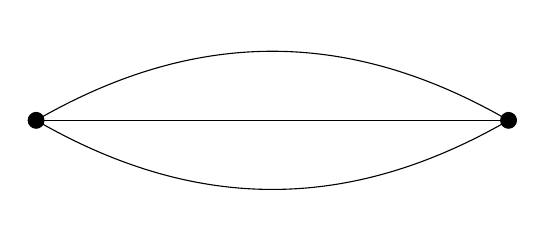
\begin{tikzpicture}
      \draw (0,0) to [out=30, in=150] (6,0) ;
      \draw (0,0) to [out=-30, in=-150] (6,0) ;
      \draw (0,0) to [out=0, in=180] (6,0) ;

      \draw [fill] (0,0) circle [radius=.1cm] ;
      \draw [fill] (6,0) circle [radius=.1cm] ;      
    \end{tikzpicture}
    \caption{The $3$-banana $B_3$}
  \end{center}
\end{figure}

\begin{prop}
  \label{prop:banana_cyclic}
  Let $B_n$ be the banana graph on $n$ edges. Then $\Jac(B_n) \simeq \Z/n\Z$.
\end{prop}

\begin{proof}
  A spanning tree on $B_n$ consists of a single edge between its
  vertices $v_1$ and $v_2$, so $B_n$ has $n$ spanning trees and
  $|\Jac(B_n)| = n$. To show that $\Jac(B_n) \simeq \Z/n\Z$, it
  suffices to find a single element of order at least $n$.

  Let $D \in \Div^0(B_n)$ be the divisor $(v_2) - (v_1)$, and consider
  $\overline{D} = [D] \in \Jac(B_n)$. For any $1 \le m < n$, the
  divisor $mD$ is $v_1$-reduced---since $v_2$ has degree $n$, it is
  impossible to fire it without sending it into debt. If $m=n$, then
  firing $v_2$ yields the zero divisor. $m\overline{D}$ is therefore
  trivial iff $m$ is a multiple of $n$, and hence $\overline{D}$ has
  order $n$ as required.
\end{proof}

\subsection{The simple graph case}
The construction given above is sufficient to show that all finite
abelian groups appear as the Jacobian of some graph. However, since
banana graphs are only realizable as a multigraphs, we might also wish
to find a construction for a simple graph $G$ with $\Jac(G) \simeq
\Z/n\Z$ for given $n$. This is (almost) always possible, by the
following proposition:

\begin{prop}
  \label{prop:cycle_cyclic}
  Let $C_n$ be the cycle graph on $n$ vertices. Then $\Jac(C_n) \simeq
  \Z/n\Z$.
\end{prop}

Each spanning tree on $C_n$ corresponds to a choice of $n-1$ edges to
include in the tree, so $\Jac(C_n)$ has order $n$ and, as before, it
suffices to find a single element of $\Jac(C_n)$ of order at least
$n$. We show that such an element exists on a wider family of graphs:

\begin{lem}
  \label{lem:2valent_path}
  Let $G$ be a biconnected graph, and suppose that for some path $P =
  \{v_1, \ldots, v_\ell\}$ on $G$, $\val(v_i) = 2$ for all $1 < i <
  \ell$. Then $\Jac(G)$ contains an element of order at least $\ell$.
\end{lem}
\begin{proof}
  Consider the divisor $D = (v_2) - (v_1)$. We claim that for any $1
  \le m < \ell$, $mD$ is equivalent to $(v_{m+1}) - (v_1)$.

  I'm going to make either a chip-firing argument or a Laplacian
  matrix argument for why this is true, but it's pretty cumbersome so
  I'll leave it for later.

  $G$ is biconnected, so there is a path from $v_1$ to $v_{m+1}$ that
  does not contain any vertex $v_i$ for $1 < i < m$. Applying the
  burning algorithm then shows that the divisor $(v_{m+1}) - (v_1)$ is
  $v_1$-reduced, and hence $m\overline{D} = m[D]$ is nontrivial for $m
  < \ell$, as required.
\end{proof}

$C_n$ is a simple graph whenever $n > 2$, so we have the following:

\begin{cor}
  Let $\Gamma$ be a finite abelian group that is not isomorphic to
  $\Z/2\Z \times H$ for any group $H$. Then there exists a simple
  graph $G$ such that $\Gamma \simeq \Jac(G)$.
\end{cor}

The rest of this section will investigate which groups $\Gamma =
\Z/2\Z \times H$ can possibly occur as the Jacobian of some simple
graph. It is known that there is no simple graph $G$ with $\Jac(G)
\simeq \Z/2\Z$ (CITE OR GIVE SHORT PROOF). We extend this result as
follows:

\begin{thm}
  \label{thm:2group}
  For any $k \ge 1$, if $G$ is a graph such that $\Jac(G) \simeq
  (\Z/2\Z)^k$, then $G$ is not simple.
\end{thm}

\begin{thm}
  \label{thm:2group_product}
  Let $H$ be a finite abelian group. There exists an integer $k_0$
  (depending on $H$) such that for all $k > k_0$, there does not exist
  a simple graph $G$ with $\Jac(G) \simeq (\Z/2\Z)^k \times H$.
\end{thm}

To prove Theorem \ref{thm:2group_product}, we will first prove it in a
special case, where $G$ is required to be biconnected. If $G$ is a
graph that is not biconnected, then by definition, there is a vertex
$v_0$ such that the subgraph $G'$ induced by $V(G) \setminus \{v_0\}$
is not connected. $G$ is the wedge sum of the connected components of
$G'$ (together with the vertex $v_0$), and so $\Jac(G)$ breaks down as
a direct product of Jacobians of subgraphs of $G$.

\begin{defn}
  Let $G$ be a graph, and let $\Gamma = \Jac(G)$. We will write $\mu(G)$
  for the maximum order of an element of $\Gamma$, and $\delta(G)$ for
  the maximum valency of a vertex in $G$. (When the graph $G$ is clear
  from context, we will simply write $\delta$ or $\mu$). 
\end{defn}

\begin{lem}
  \label{lem:delta_le_mu}
  If $G$ is biconnected, then $\delta \le \mu$.
\end{lem}
\begin{proof}
  Let $v$ be a vertex in $V(G)$ with valency $\delta$, and let $w$ be
  a vertex adjacent to $w$. Consider the divisor $D = (v) -
  (w)$, and let $m < \delta$. 

  We may apply Dhar's burning algorithm to check that $mD$ is
  $w$-reduced. Since $G$ is biconnected, there is a path from $w$ to
  each of the neighbors of $v$ that does not contain $v$, and so each
  of the neighbors of $v$ is ``burned'' by the algorithm. $v$ has more
  than $m$ distinct neighbors, so it is burned as well. Therefore,
  $m\overline{D}$ is nontrivial and $\overline{D}$ has order at least
  $\delta$.
\end{proof}

\begin{cor}
  \label{cor:genus_v_mu}
  For any biconnected graph with genus $g$ and $|V(G)| = v$,
  \begin{equation*}
    v \ge \frac{2g - 2}{\mu - 1}
  \end{equation*}
\end{cor}
\begin{proof}
  Let $e = |E(G)|$. We have 
  \begin{equation*}
    2e = \sum_{i=1}^n \val(v_i) \le \sum_{i=1}^n \delta = v \cdot \delta
    \le v \cdot \mu
  \end{equation*}
  Since $e = g + v - 1$, this gives
  \begin{equation*}
    2g - 2 \le v \cdot (\mu - 1)
  \end{equation*}
  as required.

\end{proof}

\begin{proof}[Proof of Theorem \ref{thm:2group}]
  Let $G$ be a biconnected graph with $\Jac(G) = (\Z/2\Z)^k$. By
  Corollary \ref{cor:1_valent}, we may assume without loss of
  generality that each vertex of $G$ has valency at least $2$. By
  Lemma \ref{lem:delta_le_mu}, each vertex of $G$ has valency exactly
  $2$, and $G = C_n$ for some $n$. We must have $n=2$, which means $G$
  cannot be simple.

  Now let $G$ be a graph that is not biconnected, with $\Jac(G) \simeq
  (\Z/2\Z)^k$. We proceed by induction on $k$.
  
  The base case $k=1$ is known. For $k > 1$, note that $\Jac(G) \simeq
  \Jac(G_1) \times \Jac(G_2)$ for connected subgraphs $G_1, G_2$ of
  $G$. Without loss of generality, $G_2$ is not a tree, and
  hence $\Jac(G_1) \simeq (\Z/2\Z)^{k_1}$ for $k_1 < k$. By the
  induction hypothesis, $G_1$ is not simple, and so neither is $G$.
\end{proof}

\begin{remark}
  The proof of Theorem \ref{thm:2group} also gives a complete
  characterization of any graph $G$ with $\Jac(G) \simeq
  (\Z/2\Z)^k$: in general, $G$ must be a tree with precisely $k$ of
  the edges occuring two times. We will apply this fact later, in our
  discussion of the monodromy pairing on $\Jac(G)$.
\end{remark}

\begin{figure}[H]
  \begin{center}
    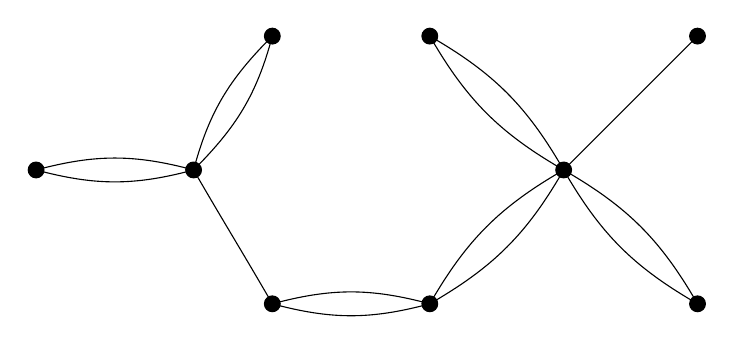
\begin{tikzpicture}

      \draw (0,0) to [out=15, in=165] (2,0) ;
      \draw (0,0) to [out=-15, in=-165] (2,0) ;

      \draw (2,0) to [out=75, in=225] (3, 1.7) ;
      \draw (2,0) to [out=45, in=255] (3, 1.7) ;

      \draw (2,0) to [out=-60, in=-240] (3, -1.7) ;

      \draw (3,-1.7) to [out=15, in=165] (5, -1.7) ;
      \draw (3,-1.7) to [out=-15, in=-165] (5, -1.7) ;

      \draw (5, -1.7) [out=60, in=210] to (6.7, 0) ;
      \draw (5, -1.7) [out=30, in=240] to (6.7, 0) ;

      \draw (6.7, 0) [out=120, in=-30] to (5, 1.7) ;
      \draw (6.7, 0) [out=150, in=-60] to (5, 1.7) ;

      \draw (6.7, 0) to (8.4, 1.7) ;

      \draw (6.7, 0) to [out=-30, in=120] (8.4, -1.7) ;
      \draw (6.7, 0) to [out=-60, in=150] (8.4, -1.7) ;

      \draw [fill] (0,0) circle [radius=.1cm] ;
      \draw [fill] (2,0) circle [radius=.1cm] ;
      \draw [fill] (3,1.7) circle [radius=.1cm] ;
      \draw [fill] (3,-1.7) circle [radius=.1cm] ;
      \draw [fill] (5,-1.7) circle [radius=.1cm] ;
      \draw [fill] (6.7, 0) circle [radius=.1cm] ;
      \draw [fill] (5,1.7) circle [radius=.1cm] ;
      \draw [fill] (8.4,1.7) circle [radius=.1cm] ;
      \draw [fill] (8.4,-1.7) circle [radius=.1cm] ;
    \end{tikzpicture}
    \caption{$\Jac(G) \simeq (\Z/2\Z)^6$}
  \end{center}
\end{figure}

We will now prove Theorem \ref{thm:2group_product}, using a similar
inductive argument on biconnected subgraphs. Throughout the following,
we will suppose that $G$ is a biconnected graph with Jacobian $\Gamma
\simeq (\Z/2\Z)^k \times H$ for some finite abelian group $H$, and
that $\mu$ is the maximum order of an element of $H$. We first
establish a bound on the genus of $G$:

\begin{lem}
  \label{lem:genus_cycle}
  If $g$ is the genus of $G$, then $g \ge k$.
\end{lem}
\begin{proof}
  For any graph $G_0$, let $h$ be the number of nontrivial invariant
  factors of $\Jac(G_0)$. Let $G_0'$ be the graph obtained by adding a
  single edge to $G_0$. We know $|h(G_0') - h(G_0)| \le 1$ (CITE
  THIS). 
%%%%%%%%%%%%%%%%%%%%%%%%%%%%%%%%%%%%%%%%%%%%%%%%%%%%%%%%%%%%%%%%%%%%%%%%%%%%%%%%%%%%%%%%

  Since a graph $G$ with genus $g$ may be constructed by adding $g$ edges
  to a spanning tree for $G$, $\Jac(G)$ has at most $g$ invariant
  factors (and thus at most $g$ factors of $\Z/2\Z$). 
\end{proof}

Applying Corollary \ref{cor:genus_v_mu} to this result gives us a
lower bound on $|V(G)|$ in terms of $k$ and $\mu$. We now establish an
upper bound on $|V(G)|$ in terms of $\mu$ and $|H|$, to achieve an
upper bound on $k$.

\begin{prop}
  \label{prop:v_bound}
  For any finite abelian group $H$, there exists an integer $v_0$
  (depending only on $H$) such that if $\Gamma = \Jac(G) \simeq (\Z/2\Z)^k
  \times H$, then $|V(G)| < v_0$.
\end{prop}

\begin{proof}
  Let $U = \{u \in V(G) : \val(u) > 2\}$, and enumerate the elements
  of $U$ as $u_0, \ldots, u_{m-1}$. We will first establish a bound on
  $m = |U|$, and then bound $|V(G)|$ in terms of $m$.
  
  Consider the set of divisors $\mathcal{U} = \{(u_i) - (u_0) : 0 \le
  i < m\}$, and write $D_i$ for $(u_i) - (u_0)$. For any $D_i, D_j \in
  \mathcal{U}$, we claim that $2D_j - 2D_i$ is $u_i$-reduced.

  We have $2D_j - 2D_i = 2(u_j) - 2(u_i)$. Since $G$ is biconnected,
  there is a path from $u_i$ to each of the neighbors of $u_j$ that
  does not contain $u_j$. Since $u_j$ has valency at least $3$, an
  iteration of the burning algorithm must burn $u_j$, and in turn the
  entire graph. Furthermore, since $2D_j - 2D_i$ is $u_i$-reduced,
  $2[D_j] \ne 2[D_i]$ for any $i \ne j$.

  Now let $\phi:\Gamma \to \Gamma$ be the map given by
  \[
  \phi(\overline{D}) = 2\overline{D}
  \] 

  We must have $|\im(\phi)| \le |H|$. In particular, if
  $\overline{\mathcal{U}} \subseteq \Gamma$ is the set of equivalence
  classes of the elements of $\mathcal{U}$, we must have
  $|\phi(\overline{\mathcal{U}})| \le |H|$, and hence $m \le |H|$ as
  well.

  We now wish to bound $|V(G)|$ in terms of $m$. To do so, we will
  consider a graph $G'$, given by the following transformation of $G$:

  \begin{enumerate}
  \item Choose some vertex of $G$ of valency $2$. Delete it, and
    draw an edge between its neighbors.
  \item Repeat until there are no 2-valent vertices remaining.
  \end{enumerate}
  %%%%%%%%%%%%%%%%%%%%%%%%%%%%%%%%%%%%%%%%%%%%%%%%%%%%%%%%%%%%%%%%%%%%%%%%%%%%%%%%%%%%%%%% 

  \begin{figure}[H]
    \begin{center}
      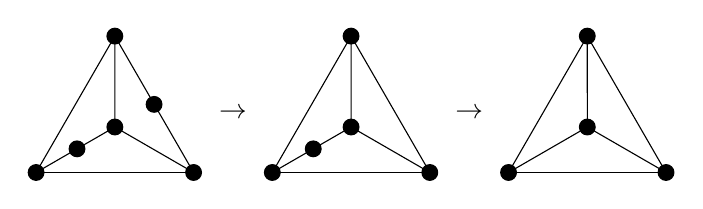
\begin{tikzpicture}

        \draw (0:0) to (60:2) ;
        \draw (0:0) to (0:2) ;
        \draw (60:2) to (0:2) ;
        \draw (0:0) to (30:1.155) ;
        \draw (0:2) to (30:1.155) ;
        \draw (60:2) to (30:1.155) ;

        \draw [fill] (0:0) circle [radius=.1cm] ;
        \draw [fill] (0:2) circle [radius=.1cm] ;
        \draw [fill] (60:2) circle [radius=.1cm] ;
        \draw [fill] (30:1.155) circle [radius=.1cm] ;
        \draw [fill] (30:.6) circle [radius=.1cm] ;
        \draw [fill] (30:1.73) circle [radius=.1cm] ;

        \draw [shift={(3,0)}] (0:0) to (60:2) ;
        \draw [shift={(3,0)}] (0:0) to (0:2) ;
        \draw [shift={(3,0)}] (60:2) to (0:2) ;
        \draw [shift={(3,0)}] (0:0) to (30:1.155) ;
        \draw [shift={(3,0)}] (0:2) to (30:1.155) ;
        \draw [shift={(3,0)}] (60:2) to (30:1.155) ;

        \draw [shift={(3,0)}][fill] (0:0) circle [radius=.1cm] ;
        \draw [shift={(3,0)}][fill] (0:2) circle [radius=.1cm] ;
        \draw [shift={(3,0)}][fill] (60:2) circle [radius=.1cm] ;
        \draw [shift={(3,0)}][fill] (30:1.155) circle [radius=.1cm] ;
        \draw [shift={(3,0)}][fill] (30:.6) circle [radius=.1cm] ;

        \draw [shift={(6,0)}] (0:0) to (60:2) ;
        \draw [shift={(6,0)}](0:0) to (0:2) ;
        \draw [shift={(6,0)}](60:2) to (0:2) ;
        \draw [shift={(6,0)}](0:0) to (30:1.155) ;
        \draw [shift={(6,0)}](0:2) to (30:1.155) ;
        \draw [shift={(6,0)}](60:2) to (30:1.155) ;

        \draw [shift={(6,0)}][fill] (0:0) circle [radius=.1cm] ;
        \draw [shift={(6,0)}][fill] (0:2) circle [radius=.1cm] ;
        \draw [shift={(6,0)}][fill] (60:2) circle [radius=.1cm] ;
        \draw [shift={(6,0)}][fill] (30:1.155) circle [radius=.1cm] ;

        \node at (2.5, .75) {$\rightarrow$} ;
        \node at (5.5, .75) {$\rightarrow$} ;

      \end{tikzpicture}
      \caption{The transformation $G \mapsto G'$}
    \end{center}
  \end{figure}

  Note that even if $G$ is simple, $G'$ need not be. It is clear,
  however, that $G$ and $G'$ have the same number of vertices with
  valency greater than $2$, and that $\delta(G) = \delta(G')$.

  By Lemma \ref{lem:delta_le_mu}, we must have that $e' = |E(G')|$ is
  at most $m \cdot \mu$ (since otherwise there would necessarily be a
  vertex of $G$ with valency greater than $\delta$). Each 2-valent
  vertex of $G$ is uniquely associated with some edge of $G'$. If
  there are more than $e' \cdot \mu$ 2-valent vertices in $G$, then at
  least $\mu$ of them are associated with a single edge of $G'$. 

  $G$ then contains a path $P$ of length greater than $\mu$, where
  each vertex of $P$ has valency $2$. This is a contradiction by Lemma
  \ref{lem:2valent_path}, so we must have 
  \[
  |V(G)| - m < m\mu^2
  \] 
  Choosing $v_0 = |H| + |H| \cdot \mu^2$ then gives $|V(G)| < v_0$, as
  required.
\end{proof}

Applying Corollary \ref{cor:genus_v_mu} and Lemma
\ref{lem:genus_cycle}, we see that for sufficiently large $k$, we must
have $|V(G)| > v_0$. This in turn implies that for sufficiently large
$k$, $(\Z/2\Z)^k \times H$ is not the Jacobian of any biconnected
graph.\\

We complete the proof of Theorem \ref{thm:2group_product} via
induction on $|H|$\footnote{We could obtain a slightly better bound by
  inducting on the number of invariant factors of $H$. This is
  slightly more cumbersome, and is left to the revisor as an
  exercise}. When $|H| = 1$ or $2$, Theorem \ref{thm:2group} gives the
bound $k_0 = 1$. For $|H| \ge 3$, there must exist (by Proposition
\ref{prop:v_bound}) an integer $k'$ such that if $k > k'$, and
$\Jac(G) \simeq (\Z/2\Z)^k \times H$, then $G$ is not biconnected.

By the induction hypothesis, for any proper subgroup $H' \subset H$,
there exists an integer $k(H')$ such that for all $k > k(H')$, no
simple graph $G'$ has $\Jac(G') \simeq (\Z/2\Z)^k \times H'$. Now,
since $H$ is finite, there are finitely many pairs of nontrivial
proper subgroups $H_1, H_2 \subset H$ such that $H_1 \times H_2 \simeq
H$. Define

\begin{equation*}
  k'' = \max\{k(H_1) + k(H_2) : H_1, H_2 \textrm{ nontrivial}, H_1
  \times H_2 \simeq H\}
\end{equation*}

Now let $k_0 = \max(k', k'')$. We wish to show that for all $k > k_0$,
if $\Jac(G) \simeq (\Z/2\Z)^k \times H$, then $G$ is not simple. Let
$G$ be a graph with this Jacobian, and let $k > k_0$.  Since $k > k'$,
$G$ is not biconnected, so it must be the wedge sum of two graphs
$G_1$ and $G_2$. There must then exist integers $k_1, k_2$ with $k_1 +
k_2 = k$ and groups $H_1, H_2$ with $H_1 \times H_2 \simeq H$ such
that

\begin{align}
  \Jac(G_1) &\simeq (\Z/2\Z)^{k_1} \times H_1 \\
  \Jac(G_2) &\simeq (\Z/2\Z)^{k_2} \times H_2
\end{align}

Without loss of generality, we may assume that neither $G_1$ nor $G_2$
is a tree, so that $\Jac(G_1)$ and $\Jac(G_2)$ are both nontrivial. In
that case, if either $H_1$ or $H_2$ were trivial, then $G_1$
(resp. $G_2$) would have Jacobian isomorphic to $(\Z/2\Z)^k$ for $k >
0$, implying that at least one of $G_1$ or $G_2$ is not simple.

Finally, since $k_1 + k_2 = k > k'' \ge k(H_1) + k(H_2)$, we must have
that either $k_1 > k(H_1)$ or $k_2 > k(H_2)$. Then either $G_1$ or
$G_2$ is not simple, so that $G$ is not simple, as required.

\subsection{Further queries} 

Analysis of the proof of Theorem \ref{thm:2group_product} suggests
that, if $H$ is cyclic of prime power order, $k_0(H)$ is
$O(|H|^4)$. In practice, it seems that much better bounds should
hold. For instance, no simple graph $G$ has yet been found where
$\Jac(G) \simeq (\Z/2\Z)^k \times H$ for any $k > |H|$.

In some cases, it is possible to directly verify that certain groups
do not arise as the Jacobian of any simple graph. We note that, for
given $m$, while there are infinitely many isomorphism classes of
simple graphs with fewer than $m$ spanning trees, at most finitely
many of these classes represent 2-edge-connected graphs. (THIS MIGHT
NEED A PROOF).

Lemma \ref{prop:wedge_product} tells us that any graph $G$ may be
uniquely associated to some 2-edge-connected graph with identical
Jacobian. For a given group $H$, it is possible to compute the
Jacobian of all 2-edge-connected simple graphs with at most $|H|$
spanning trees, and verify that $H$ does or does not occur. 

Computer searches of this nature have led to the following:

\begin{thm}
  The groups $\Z/2\Z \times \Z/4\Z$, $(\Z/2\Z)^2 \times \Z/4\Z$, and
  $\Z/2\Z \times (\Z/4\Z)^2$ are not isomorphic to the Jacobian of any
  simple graph.
\end{thm}

It is also of interest that the key fact in the proof of the
nonoccurence of groups with many factors of $\Z/2\Z$ seems to be the
requirement that $G$ is biconnected, rather than that $G$ is
simple. This, together with the discovery that the Jacobians of
``most'' graphs are cyclic (CITE STUFF), suggests the following:

\begin{conj}
  Let $G$ be a biconnected graph. For any $n$, there exists $k_0$ such
  that if $k > k_0$, $\Jac(G) \not\simeq (\Z/n\Z)^k$.
\end{conj}

Finally, we note that when $\Jac(G) \simeq (\Z/n\Z)^k \times H$ for
some finite abelian group $H$, $k$ is necessarily bounded above by the
genus of $G$. The next section will consider certain circumstances
under which this bound can be achieved, and also say some things about
metric graphs.

\section{Relationship to Jacobians of Metric Graphs}
\begin{lem}
  \label{lem:jac_generators}
  Let $G$ be a graph. $\Jac(G)$ is generated by the set \[\{[(v) -
  (w)]: \{v, w\} \in E(G)\}\]
\end{lem}

\begin{proof}
  In general, $\Div^0(G)$ is generated by divisors of the form $(v_a)
  - (v_b)$ for $v_a, v_b \in V(G)$. Since $G$ is connected, any such
  divisor may be represented as a sum of divisors of the form $(v) -
  (w)$ for adjacent $v$ and $w$ (formal proof can be given if
  necessary). Therefore the Jacobian is generated by the equivalence
  classes of these divisors.  
\end{proof}

\section{The monodromy pairing on the Jacobian}

The Jacobian of a finite graph is endowed with a natural monodromy
pairing. Since it is possible to classify all finite abelian groups
with pairing, it is worth considering which groups \emph{with pairing}
occur as the Jacobian of some graph. This section will investigate
this question.

\begin{note}
  Throughout the following, unless otherwise noted, we will always use
  the word ``group'' to mean ``group \emph{with pairing},''
  ``isomorphism'' and ``$\simeq$'' to mean an isomorphism of groups
  with pairing, and $\oplus$ to denote the orthogonal sum on groups
  with pairing. For a graph $G$, we will take $\Jac(G)$ to mean the
  Jacobian of $G$ with its associated monodromy pairing.
\end{note}

Our main result will be the following:

\begin{thm}
  Let $\Gamma$ be a finite abelian group of odd order, not isomorphic
  to $(\Z/p\Z) \times H$ for any prime $p \equiv 1 \pmod {24}$ and
  group $H$. Then there exists a graph $G$ such that
  \[
  \Jac(G) \simeq \Gamma
  \]
\end{thm}

Under the assumption of the Generalized Riemann Hypothesis, this
result can be strengthened:
\begin{thm}
  Let $\Gamma$ be a finite abelian group of odd order. If the
  Generalized Riemann Hypothesis holds, then there exists a graph $G$
  such that 
  \[
  \Jac(G) \simeq \Gamma
  \]
\end{thm}

As in the case of groups without pairing, we will take advantage of
the fact that the wedge sum of two graphs corresponds to a product
operation on the Jacobians of those graphs. In this case, the
``product'' will be the orthogonal sum:

\begin{prop}
  \label{prop:wedge_sum}
  Let $G_1$, $G_2$ be graphs. Then $\Jac(G_1 \vee G_2) \simeq
  \Jac(G_1) \oplus \Jac(G_2)$. 
\end{prop}
\begin{proof}
  DANIEL MITROPOLSKY WHY HAVE YOU FORSAKEN US
\end{proof}

The problem is now reduced to the following: given a prime $p$, a
positive integer $r$, and a pairing $\pair{\cdot}{\cdot}$ on
$\Z/p^r\Z$, we wish to find a graphs $G$ such that $\Jac(G) \simeq
(\Z/p^r\Z, \pair{\cdot}{\cdot})$.

Section \ref{sec:jacobians} gave a construction for graphs with any
desired Jacobian, but we require a way to construct graphs whose
Jacobian is associated with a particular pairing. We provide two such
constructions below:

\begin{defn}
  Let $S = \{s_1, \ldots, s_m\}$ be a multiset of positive
  integers. $B_S$, the \emph{subdivided banana graph of $S$}, is the
  graph obtained by subidividing the $i$th edge of $B_m$ by $s_i-1$
  vertices. 
\end{defn}

\begin{defn}
  Let $S = \{s_1, \ldots, s_m\}$ be a multiset of positive
  integers. $C_S$, the \emph{stupidly named cycle graph of $S$}, is
  the graph obtained giving the $i$th edge of $C_m$ multiplicity
  $s_i$.
\end{defn}

We will use the following notation for particular integer quantities
on a multiset $S$:
\begin{defn}
  Let $S = \{s_1, \ldots, s_m\}$. Define
  \begin{align*}
    P(S) &= \prod_{i=1}^ms_i\\
    R(S) &= \sum_{i=1}^mP(S)s_i^{-1}
  \end{align*}
\end{defn}

\begin{prop}
  \label{prop:banana_pairing}
  Let $S$ be a multiset of positive integers such that $R(S) = p^r$ for an odd prime $p$ and integer $r$, such that some divisor is not $p^{r-1}$ torsion. Then 
  \begin{equation*}
    \Jac(B_S) \simeq (\Z/p^r\Z, \pair{\cdot}{\cdot})
  \end{equation*}
  where $\pair{\cdot}{\cdot}$ is the pairing on $\Z/p^r\Z$ given by
  \begin{equation*}
    \pair{x}{y} = \frac{P(S)xy}{p^r}
  \end{equation*}
\end{prop}
\begin{proof}
 First note that $B_{S}$ has $p^r$ trees. Of the $m$ edges before subdividing choose $1$ to form the tree. Let this be the $i$-th edge. Upon subdividing all of the $s_{i}$ subdivided edges in the original $i$-th edge must be present. We must eliminate $1$ edge formed from subdivision from the each of the remaining $m-1$ original edges we must choose to eliminate $1$ edge from each. There are $s_{j}$ choices of ways to eliminate an edge formed from by subdivision from the original $j$-th edge. Taking the product of these and summing over $i$s gives $\sum^{m}_{i=1}s_{1}\dots \hat{s_{i}} \dots s_{m}=R(S)$.
 
 By the Matrix Tree Theorem group is of order $p^{r}$. Since each element is $p^{t}$ torsion for $0\le t\le r$ and there exists an element that is not $p^{r-1}$ torsion that element must be $p^{r}$ torsion. Since there exists an element that is $p^r$ torsion and the group is of order $p^r$ the group must be isomorphic to $\Z/p^{r}/Z$.
 
 To see that the pairing on the group is isomorphic to $\frac{P(S)xy}{p^r}$ take the two vertices on the original banana. Taking a smooth piecewise linear function such that between two adjacent vertices on the $i$-th edge their difference is $s_{1}\dots \hat{s_{i}} \dots s_{m}$ and this increases linearly we see that the difference between the two original edges is $P(S)$. Furthermore we see that this is same no matter which of the $m$ original edges we choose as the difference will always be $s_{1}\dots \hat{s_{i}} \dots s_{m}\cdot s_{i}$, and that out of the negative of the two edges the slope is $R(S)$ and the slope into the positive edge is $R(S)$. Thus this function satisfies the conditions to be the monodromy pairing, implying that $\Jac(B_S) \simeq (\Z/p^r\Z, \pair{\cdot}{\cdot})$
\end{proof}

If $p$ is odd, there are only two such pairings. In this case, our
goal is to find graphs $G_1$, $G_2$ such that $\Jac(G_1) \simeq
(\Z/p^r\Z, \mathfrak{r})$ and $\Jac(G_2) \simeq (\Z/p^r\Z,
\mathfrak{n})$, where $\mathfrak{r}$ and $\mathfrak{n}$ represent the
residue and nonresidue pairings on $\Z/p^r\Z$, respectively. 

\begin{prop}
  \label{prop:banana_residue}
  Let $B_{p^r}$ be the banana graph on $p^r$ edges. Then
  $\Jac(B_{p^r}) \simeq (\Z/p^r\Z, \mathfrak{r})$.
\end{prop}

\begin{proof}

It is easy to check that there is one nontrivial invariant factor in the Smith normal form of the laplacian matrix of $B_{p^r}$, which is equal to $\left(\begin{array}{cc}p^{r}&-p^r\\-p^r&p^r\end{array}\right)$.

 To see that $B_{p^r}$ has the residue pairing, it is sufficient to take the pairing of $\left[\begin{array}{c}-1\\1\end{array}\right]$ with itself. As noted in %Shokrieh
the monodromy pairing is given by $\pair{\overline{D_1}}{\overline{D_{2}}}=[D_1]^{T}\digamma[D_2]$, where $\digamma$ is a generalized inverse of the laplacian. One such generalized inverse is $\digamma=\frac{1}{p^{r}}\left(\begin{array}{cc}0&0\\0&1\end{array}\right)$. Thus pairing $\left[\begin{array}{c}-1\\1\end{array}\right]$ with itself gives $\frac{1}{p^{r}}$. Since $1$ is always a residual, $\Jac(B_{p^r}) \simeq (\Z/p^r\Z, \mathfrak{r})$.

(CITE STUFF BY SHOKRIEH)
\end{proof}

\begin{lem}
 \label{lemma:2-group iso}
 If $a\equiv b\pmod 8$ for $a,b$ odd then
 \begin{equation}
  \frac{axy}{2^{r}}\simeq  \frac{bxy}{2^{r}}
 \end{equation}
  are isomorphic as pairings on $\Z/2^r\Z$ for $r\ge3$
\end{lem}
\begin{proof}
 Note that isomorphisms of pairing are derived from group isomorphisms. All isomorphisms $\phi$ on cyclic groups of order $2^{r}$ are of the form $\phi:x\to cx$ with $c$ odd. Let $\Phi$ be an isomorphism of pairings. Then $\Phi\pair{x}{y}=\pair{\phi(x)}{\phi(y)}$ for some $\phi$. Thus $\frac{axy}{2^{r}}$ is isomorphic to $\frac{bxy}{2^{r}}$ if  $ac^{2}\equiv b\pmod 2^{r}$ for some $c$. Since $a\equiv b\pmod 8$ and $c^{2}\equiv 1\pmod 8$ for all odd $c$. Since there are only $4$ isomorphism classes of pairings on $\Z/2^r\Z$ for $r\ge3$ %shokrieh
 $\frac{axy}{2^{r}}\simeq  \frac{bxy}{2^{r}}$ as there are only $4$ odd numbers modulo $8$.
\end{proof}

\begin{defn}
 Let $\mathcal{P}_{2}$ denote be the semigroup of
isomorphism classes of non degenerate symmetric bilinear pairings on
finite abelian 2-groups, under orthogonal direct sum.
%rewrite so as not to copy from Miranda

\end{defn}

 \begin{prop} $\mathcal{P}_{2}$ is generated by the following
pairings:
  
   \[ \AP \text{ on } \Z/2^{n}\Z, r\ge 1; \langle 1,
1\rangle=\frac{1}{2^{n}}
   \]
   \[ \BP \text{ on } \Z/2^{n}\Z, r\ge 2; \langle 1,
1\rangle=\frac{-1}{2^{n}}
   \]
   \[ \CP \text{ on } \Z/2^{n}\Z, r\ge 3; \langle 1,
1\rangle=\frac{5}{2^{n}}
   \]
   \[ \DP \text{ on } \Z/2^{n}\Z, r\ge 3; \langle 1,
1\rangle=\frac{-5}{2^{n}}
   \]
   \[ \EP \text{ on } \Z/2^{n}\Z\times\Z/2^{n}\Z, r\ge 1; \langle
e_{i}, e_{j}\rangle=\begin{cases}0&\mbox{if } i=j\\
\frac{1}{2^{n}}&\mbox{if } i\neq j\end{cases}
   \]
   \[ \FP \text{ on } \Z/2^{n}\Z\times\Z/2^{n}\Z, r\ge 2; \langle
e_{i}, e_{j}\rangle=\begin{cases}\frac{1}{2^{n-1}}&\mbox{if } i=j\\
\frac{1}{2^{n}}&\mbox{if } i\neq j\end{cases}
   \]
   
where $\{e_{1}, e_{2}\}$ generate $\Z/2^{n}\Z\times\Z/2^{n}\Z$ in the
last two cases.
 \end{prop}
 \begin{proof} See [Mir]
 \end{proof}

 \begin{thm} For each of $\AP$, $\BP$, $\CP$, $\DP$ there exists a
graph $G$ such that the monodromy pairing on $G$ is the desired
pairing.
 \end{thm}

\begin{proof}
 Case 1: $\AP$. $B_{2^{n}}$ is cyclic of order $2^{n}$ has pairing
$\AP$. This follows from \ref{prop:banana_residue}.

%A pairing 
\begin{center}
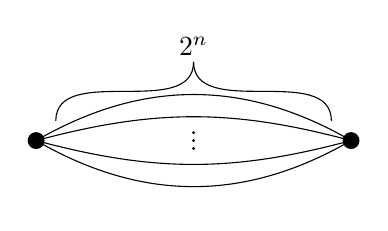
\begin{tikzpicture}

\draw (0,0) to [out=330,in=210] (4,0) ;
\draw (0,0) to [out=345,in=195] (4,0) ;
\draw (0,0) to [out=15,in=165] (4,0) ;
\draw (0,0) to [out=30,in=150] (4,0) ;

\draw [fill] (2,.1) circle [radius=0.01cm] ;
\draw [fill] (2,0) circle [radius=0.01cm] ;
\draw [fill] (2,-.1) circle [radius=0.01cm] ;

\draw (.25,.25) to [out=90,in=-90] (2,1) ;
\draw (3.75,.25) to [out=90,in=-90] (2,1) ;

\draw [fill] (4,0) circle [radius=0.1cm] ;
\draw [fill] (0,0) circle [radius=0.1cm] ;

\node at (2, 1.2) {$2^{n}$} ;

\end{tikzpicture}
\end{center}

  
   Case 2: $\BP$. The cycle graph on $2^{n}$ vertices has pairing
$\BP$.
%%%%we should prove that the pairing on the cycle is always n-1/n%%%%%%%%%

%B pairing check the labeling
\begin{center}
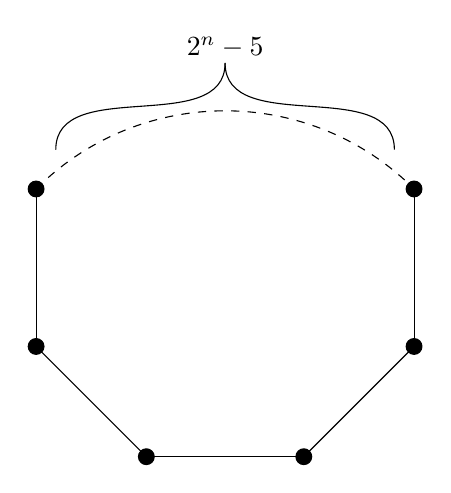
\begin{tikzpicture}

\draw (0,0) to (0,-2) ;
\draw (0,-2) to (1.4,-3.4) ;
\draw (1.4,-3.4) to (3.4,-3.4) ;
\draw (3.4,-3.4) to (4.8,-2) ;
\draw (4.8,-2) to (4.8, 0) ;
\draw [dashed] (0,0) to [out=45, in=135] (4.8,0) ;

\draw [fill] (4.8,0) circle [radius=0.1cm] ;
\draw [fill] (0,0) circle [radius=0.1cm] ;
\draw [fill] (0,-2) circle [radius=0.1cm] ;
\draw [fill] (1.4,-3.4) circle [radius=0.1cm] ;
\draw [fill] (3.4,-3.4) circle [radius=0.1cm] ;
\draw [fill] (4.8,-2) circle [radius=0.1cm] ;

\draw (.25,.5) to [out=90,in=-90] (2.4,1.6) ;
\draw (4.55,.5) to [out=90,in=-90] (2.4,1.6) ;

\node at (2.4, 1.8) {$2^n-5$} ;


\end{tikzpicture}
\end{center}
  
   Case 3a: For $n$ odd take $\left\{1, 2,\frac{2^{n}-2}{3}\right\}_{b}$. One can check that the divisor $D=v-w$ where $w$ is a trivalent vertex and $v$ is the adjacent vertex
on edge that was subdivided $\frac{2^{n}-2}{3}$ times, has order, by using the slope
definition of the monodromy pairing by defining the function such that all slopes are increasing in the direction of $v$ and decreasing from $w$. This results in the linear equations
  \begin{equation*}
a+b+c=2^{t}
  \end{equation*}
  \begin{equation*}
a=2b
  \end{equation*}
  \begin{equation*}
a+\left(\frac{2^{n}-2}{3}-1\right)(a+b)=c
  \end{equation*}
where $a$ is the slope on the undivided edge, $b$ is the
slope the edges formed from the edge that was subdivided once, and $c$ is the slope
on the edge between $v$ and $w$. Solving the equation gives
\begin{equation*}
2^{n}a=2^{t}
\end{equation*}
Since $t$ is at most $n$ and $t=n$ is the only solution such that $a$ has nonnegative integer value the order of this element must be $2^{n}$. Furthermore, $c=2^{n}-3$, implying that the pairing of $D$ with itself is $\frac{2^{n}-3}{2^{n}}$ which by \ref{lemma:2-group iso} is isomorphic to the $\CP$ pairing.

$c=2^{n}-3$. Thus the pairing is $\frac{2^{n}-3}{2^{n}}$, which is
isomorphic to $\CP$ by \ref{lemma:2-group iso}.

%C pairing n odd
\begin{center}
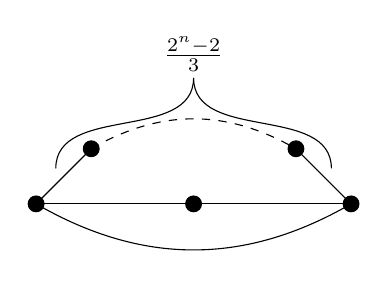
\begin{tikzpicture}

\draw (0,0) to (4,0) ;
\draw (0,0) to [out=-30, in=-150] (4,0) ;
\draw (0,0) to (.7,.7) ;
\draw (3.3,.7) to (4,0) ;
\draw [dashed] (.7,.7) to [out=30, in=150] (3.3,.7) ;

\draw [fill] (0,0) circle [radius=.1] ;
\draw [fill] (4,0) circle [radius=.1] ;
\draw [fill] (2,0) circle [radius=.1] ;
\draw [fill] (.7,.7) circle [radius=.1] ;
\draw [fill] (3.3,.7) circle [radius=.1] ;

\draw (.25,.45) to  [out=90, in=-90] (2,1.6) ;
\draw (3.75,.45) to  [out=90, in=-90] (2,1.6) ;

\node at (2,1.9) {$\frac{2^{n}-2}{3}$} ;

\end{tikzpicture}
\end{center}
    
    Case 3b: For $n$ even take $\left\{1,1,1,
\frac{2^{n}-1}{3}\right\}_{b}$. To check that the divisor
$D=v-w$ where $w$ is a trivalent vertex and $v$ is the adjacent vertex
on edge subdivided $\frac{2^{n}-1}{3}$ times  has order $2^{n}$, by using the slope
definition of the monodromy pairing by defining the function such that all slopes are increasing in the direction of $v$ and decreasing from $w$.  This gives the linear equations 
\begin{equation*}
a+b+c+d=2^{t}
\end{equation*}
\begin{equation*}
a=b=c
\end{equation*}
\begin{equation*}
a+\left(\frac{2^{n}-1}{3}-1 \right)(a+b+c)=d
\end{equation*}
where $a$ is the slope on one of the undivided edges
$b$ is the slope on another of the undivided edges,  $c$ is the
slope on the third undivided edge and $d$ is the slope on
the edge between $v$ and $w$.
This results in the equation 
\begin{equation*}
2^na=2^t
\end{equation*}
Since $t$ is at most $n$ and $t=n$ is the only solution such that $a$ has nonnegative  integer value the order of this element must be $2^{n}$. Furthermore $d=2^{n}-3$ implying that the pairing of $D$ with itself is $\frac{2^{n}-3}{2^{n}}$, which isisomorphic to $\CP$ by  \ref{lemma:2-group iso}.

%C pairing n even
\begin{center}
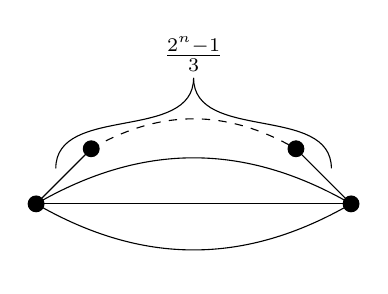
\begin{tikzpicture}

\draw (0,0) to (4,0) ;
\draw (0,0) to [out=-30, in=-150] (4,0) ;
\draw (0,0) to [out=30, in=150] (4,0) ;
\draw (0,0) to (.7,.7) ;
\draw (3.3,.7) to (4,0) ;
\draw [dashed] (.7,.7) to [out=30, in=150] (3.3,.7) ;

\draw [fill] (0,0) circle [radius=.1] ;
\draw [fill] (4,0) circle [radius=.1] ;

\draw [fill] (.7,.7) circle [radius=.1] ;
\draw [fill] (3.3,.7) circle [radius=.1] ;

\draw (.25,.45) to  [out=90, in=-90] (2,1.6) ;
\draw (3.75,.45) to  [out=90, in=-90] (2,1.6) ;

\node at (2,1.9) {$\frac{2^{n}-1}{3}$} ;

\end{tikzpicture}
\end{center}
    
    Case 4a: For odd $n$ take $\left\{1, 2,
\frac{2^{n}-2}{3}\right\}_{c}$. To check that the divisor
$D=v-w$ where $w$ is the vertex with degree has $\frac{2^{n}+4}{3}$ and
$v$ is the vertex with degree has $\frac{2^{n}+1}{3}$ has order
$2^{n}$ one can use the slope definition of the monodromy pairing. Taking the piecewise linear function such that the slopes go away from $w$ and towards $v$ one
obtains the following linear equations,
\begin{equation*}
\frac{2^{n}-2}{3}a+2b=2^{t}
\end{equation*}
\begin{equation*}
a=3b
\end{equation*}
where $a$ is slope on set of $\frac{2^{n}-2}{3}$ edges, and
$b$ is slope on the doubled edges. Since $t$ is at most $n$ and $t=n$ is the only solution such that $b$ has nonnegative integer value the order of this element must be $2^{n}$. This also implies that the pairing of $D$ with itself is $\frac{3}{2^{n}}$, as the equations have solution $a=3$. This pairing is isomorphic to
$\DP$ by  \ref{lemma:2-group iso}.

%D pairing n odd
\begin{center}
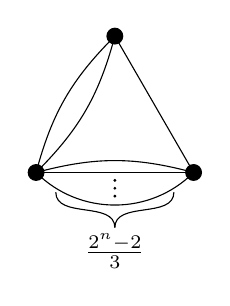
\begin{tikzpicture}

\draw (0:0) [out=45, in=-105] to (60:2) ;
\draw (0:0) [out=75, in=-135] to (60:2) ;
\draw (0:0) [out=15, in=165] to (0:2) ;
\draw (0:0) [out=0, in=180] to (0:2) ;
\draw (0:0) [out=-45, in=-135] to (0:2) ;
\draw (60:2) to (0:2) ;

\draw [fill] (1, -.3) circle [radius=.01] ;
\draw [fill] (1, -.2) circle [radius=.01] ;
\draw [fill] (1, -.1) circle [radius=.01] ;

\draw (.25,-.25) [out=-90, in=90] to (1,-.7) ;
\draw (1.75,-.25) [out=-90, in=90] to (1,-.7) ;

\draw [fill] (0, 0) circle [radius=.1] ;
\draw [fill] (0:2) circle [radius=.1] ;
\draw [fill] (60: 2) circle [radius=.1] ;

\node at (1, -1) {$\frac{2^{n}-2}{3}$} ;

\end{tikzpicture}
\end{center}
    
    Case 4b: For even $n$ take $\left\{1, 1, 1,
\frac{2^{n}-1}{3}\right\}$. To check that the divisor $D=v-w$,
where $w$ is one of the vertices with degree $\frac{2^{n}+2}{3}$
and $v$ is the other vertex with degree $\frac{2^{n}+2}{3}$, has
order $2^{n}$, use the slope definition of the monodromy pairing. Taking the piecewise linear function such that the slopes are increasing towards $w$ and away from $v$, one arrives at the linear equations
\begin{equation*}
b+ \frac{2^{n}-1}{3}a=2^{t}
\end{equation*}
\begin{equation*}
3b=a
\end{equation*}
where $a$ is the slope on edge copied $\frac{2^{n}-1}{3}$ times, and $b$
is slope on the edges that aren't copied. Since $t$ is at most $n$ and $t=n$ is the only solution such that $b$ has nonnegative integer value the order of this element must be $2^{n}$. This also implies that the pairing of $D$ with itself is $\frac{3}{2^{n}}$, as the equations have solution $a=3$. This pairing is isomorphic to
$\DP$ by  \ref{lemma:2-group iso}.

%D pairing n even
\begin{center}
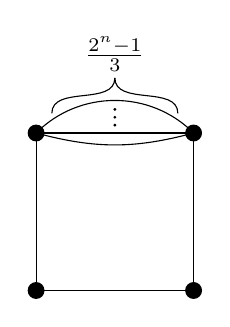
\begin{tikzpicture}

\draw (0,0) to (0,2) ;
\draw (0,0) to (2,0) ;
\draw (2,0) to (2,2) ;
\draw (0,2) to (2,2) ;
\draw (0,2) to [out=-15, in=-165] (2,2) ;
\draw (0,2) to [out=45, in=135] (2,2) ;

\draw [fill] (1, 2.1) circle [radius=.01] ;
\draw [fill] (1, 2.2) circle [radius=.01] ;
\draw [fill] (1, 2.3) circle [radius=.01] ;

\draw (.2,2.25) [out=90, in=-90] to (1,2.7) ;
\draw (1.8,2.25) [out=90, in=-90] to (1,2.7) ;

\node at (1, 3) {$\frac{2^{n}-1}{3}$} ;

\draw [fill] (0,0) circle [radius=.1] ;
\draw [fill] (2,2) circle [radius=.1] ;
\draw [fill] (2,0) circle [radius=.1] ;
\draw [fill] (0,2) circle [radius=.1] ;

\end{tikzpicture}
\end{center}
\end{proof}

\begin{prop}
\label{prop: E_2}
\end{prop}

%It's picture time motherfuckers
%C_{4}
\begin{center}
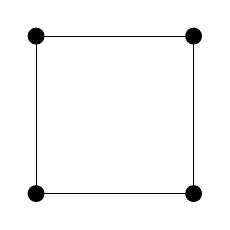
\begin{tikzpicture}

\draw (0,0) to (0,2) ;
\draw (0,0) to (2,0) ;
\draw (2,0) to (2,2) ;
\draw (0,2) to (2,2) ;

\draw [fill] (0,0) circle [radius=.1] ;
\draw [fill] (2,2) circle [radius=.1] ;
\draw [fill] (2,0) circle [radius=.1] ;
\draw [fill] (0,2) circle [radius=.1] ;

\end{tikzpicture}
\end{center}

%B_{4}
\begin{center}
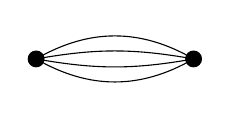
\begin{tikzpicture}

\draw (0,0) to [out=10, in=170] (2,0) ;
\draw (0,0) to [out=-10, in=-170] (2,0) ;
\draw (0,0) to [out=30, in=150] (2,0) ;
\draw (0,0) to [out=-30, in=-150] (2,0) ;

\draw [fill] (0,0) circle [radius=.1] ;
\draw [fill] (2,0) circle [radius=.1] ;

\end{tikzpicture}
\end{center}

\begin{center}
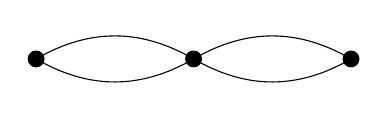
\begin{tikzpicture}

\draw (0,0) to [out=30, in=150] (2,0) ;
\draw (0,0) to [out=-30, in=-150] (2,0) ;
\draw (2,0) to [out=30, in=150] (4,0) ;
\draw (2,0) to [out=-30, in=-150] (4,0) ;

\draw [fill] (0,0) circle [radius=.1] ;
\draw [fill] (2,0) circle [radius=.1] ;
\draw [fill] (4,0) circle [radius=.1] ;

\end{tikzpicture}
\end{center}

\end{document}